\documentclass[tikz]{standalone}

\usepackage{fontspec}
\usepackage{unicode-math}
\usetikzlibrary{arrows.meta,positioning,shapes}
\setmainfont{TeX Gyre Pagella}
\setmathfont{TeX Gyre Pagella Math}
\setsansfont[Scale=0.95]{Clear Sans}
\setmonofont[
  Scale=1.05,
  UprightFeatures={SmallCapsFont=LMMonoCaps10-Regular},
  ItalicFeatures={SmallCapsFont=LMMonoCaps10-Oblique},
]{Latin Modern Mono}
% Patch for modern versions of fontspec:
\let\ttfamilyinline\relax
\newfontfamily\ttfamilyinline{Latin Modern Mono Prop}
% Adjust tikz settings:
\tikzset{
  > = {Stealth[length=2.8pt .8, inset'=0pt .575, width'=0pt 1.55, line join=round, sep]},
  normal linewidth/.style = semithick,
}


\usetikzlibrary{calc}

\begin{document}
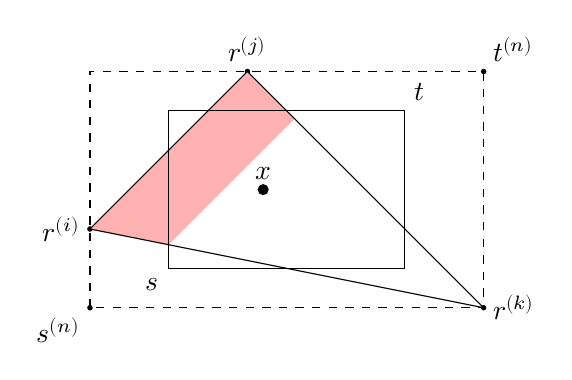
\begin{tikzpicture}[scale=1]
  \coordinate (min) at (0, 0);
  \coordinate (max) at (5, 3);
  \coordinate (alpha) at (2.2, 1.5);
  \coordinate (ri) at (0, 1);
  \coordinate (rj) at (2, 3);
  \coordinate (rk) at (5, 0);

  \node[below left] at (min) {$s^{(n)}$};
  \node[above right] at (max) {$t^{(n)}$};
  \node[above] at (alpha) {$x$};
  \node[left] at (ri) {$r^{(i)}$};
  \node[above] at (rj) {$r^{(j)}$};
  \node[right] at (rk) {$r^{(k)}$};

  \fill (min) circle (1pt);
  \fill (max) circle (1pt);
  \fill (alpha) circle (2pt);
  \fill (ri) circle (1pt);
  \fill (rj) circle (1pt);
  \fill (rk) circle (1pt);

  \fill[red!30] (ri) -- ($(rk)!0.8!(ri)$) -- ($(rk)!0.8!(rj)$) -- (rj) -- cycle;

  \draw[dashed] (min) rectangle (max);
  \draw (1, 0.5) node[below left] {$s$} rectangle (4, 2.5) node[above right] {$t$};
  \draw (ri) -- (rj) -- (rk) -- cycle;
\end{tikzpicture}
\end{document}


